\begin{frame}{Open data}{Definition}
    \begin{block}{Open data}
        \textit{``Open data is data that can be freely used, re-used and redistributed by anyone - subject only, at most, to the requirement to attribute and share alike''}.
    \end{block}
    \pause
    \begin{figure}
        \centering
        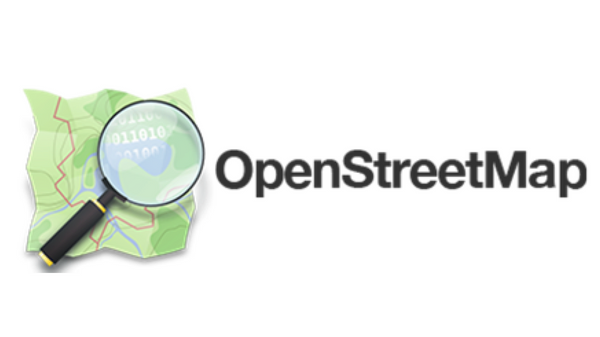
\includegraphics[width=.6\textwidth,height=.4\textwidth]{img/OSM.png}
        % \caption{Open data}
        % \label{fig:arOv}
    \end{figure}
\end{frame}

\begin{frame}{Open data}{Properties}
    \begin{itemize}
        \setbeamercovered{transparent}
        \onslide<1->{\item[+] Technically open:
              \begin{itemize}
                  \uncover<2-> {
                  %   \item The citizens access to all unrestricted data sets easily.
                  \item Accessing to data sets: unrestricted, easy.
                        }
                        \uncover<3-> {
                        % \item Data sets are available for downloading in multiple formats readable by computers.
                  \item Data formats: computer-readable.
                        }
                        % \uncover<4-> {\item The Open API provides the citizens with access to the data sets.}
              \end{itemize}}
              \pause
              \pause
              \pause
              %   \pause
              \onslide<4->{\item[+] Legally open:
              \begin{itemize}
                  \uncover<5-> {\item No restrictions on use and/or redistribution.}
                        % For example, citizens can use the data sets for either commercial or non-commercial purposes
                        % \uncover<6-> {\item Data sets are available under an open license.}
              \end{itemize}}
    \end{itemize}
    \uncover<6->{
        \begin{figure}
            \centering
            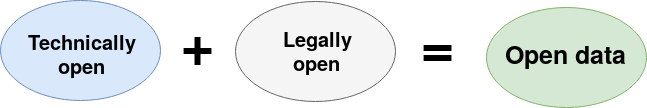
\includegraphics[width=.8\textwidth,height=.2\textwidth]{img/techleg.png}
            % \caption{Open data}
            % \label{fig:arOv}
        \end{figure}
    }
\end{frame}

\begin{frame}{Open data}{Benefits}
    % The \textit{Open data} is expected to bring a lot of benefits to:
    \vspace{0.3cm}
    \begin{columns}
        \setbeamercovered{transparent}
        \onslide<1->{
            \begin{column}{0.5\textwidth}
                +The government:
                \begin{itemize}
                    \uncover<2->{\item Improving transparency and publicity.}
                          \uncover<3->{\item Reducing the government operation cost.}
                \end{itemize}
            \end{column}}
        % \only<1-3>{
        %     \begin{column}{0.5\textwidth}
        %     \end{column}}
        \pause
        \pause
        \pause
        \onslide<4->{
            \begin{column}{0.5\textwidth}
                +The citizens:
                \begin{itemize}
                    \uncover<5->{\item Monitoring the government operation.}
                          \uncover<6->{\item Accessing to larger data resources.}
                \end{itemize}
            \end{column}}
    \end{columns}
    \uncover<7->{
        \begin{figure}
            \centering
            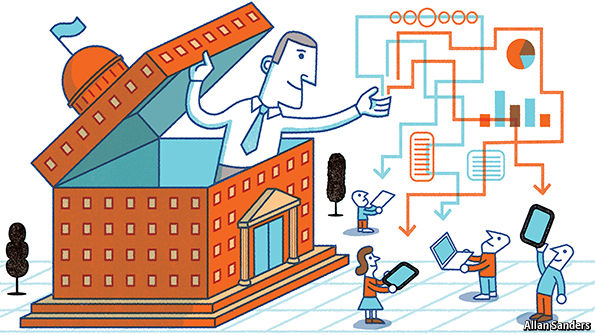
\includegraphics[width=.6\textwidth,height=.25\textwidth]{img/opendata.jpg}
            % \caption{Open data}
            % \label{fig:arOv}
        \end{figure}}
\end{frame}

\begin{frame}{Open data}{Security issues}
    % \begin{block}{Security analysis of open data}
    \setbeamercovered{transparent}
    \begin{itemize}
        \onslide<1->{\item In terms of the law:
              % it must be ensured that there is no legal violation, no disclosure of economic secrets, personal information and especially information on infrastructure.
              \begin{itemize}
                  \item<2-> no legal violation;
                  \item<3-> no disclosure of economic secrets;
                  \item<4-> no leak of personal information;
                  \item<5-> no publication of information on infrastructure.
              \end{itemize}
              }
              \pause
              \pause
              \pause
              \pause
              \pause
              \onslide<6->{\item  In terms of the technical:
              %    open data systems need to ensure  the  availability  and  integrity  of  data.
              \begin{itemize}
                  \item<7-> ensuring the availability and integrity of data.
              \end{itemize}
              }
    \end{itemize}
    % \end{block}
\end{frame}

\begin{frame}{Blockchain}{Definition}
    \begin{block}{Blockchain}
        % A \textbf{blockchain} is an electronic ledger that stores encrypted, authenticated and shared events in the format of \textit{transactions} in a decentralized network
        %  using consensus protocols.
        A \textbf{blockchain} is a growing list of records, called blocks, that are linked using cryptography. Each block contains a cryptographic
        hash of the previous block, a timestamp, and transaction data.
    \end{block}
    % \vspace{0.5cm}
    \begin{columns}
        \onslide<2->{
            \begin{column}{0.6\textwidth}
                \begin{figure}
                    \centering
                    \includegraphics<2->[width=0.9\textwidth,height=.4\textwidth]{img/blockchain.png}
                    % \caption{Blockchain}
                    % \label{fig:arOv}
                \end{figure}
            \end{column}
        }
        \onslide<3->{
            \begin{column}{0.4\textwidth}
                Types of blockchain:
                \begin{itemize}
                    \item<4-> Public blockchain.
                    \item<5-> Private blockchain.
                    \item<6-> Consortium blockchain.
                \end{itemize}
            \end{column}
        }
    \end{columns}
\end{frame}
\begin{frame}{Hyperledger Fabric}{Definition}
    % \begin{block}{
    Hyperledger Fabric:
    % }
    \begin{itemize}
        \setbeamercovered{transparent}
        \uncover<2->{
        % \item Hyperledger Fabric is a \textbf{private blockchain} developed and maintained by Linux Foundation and IBM Corporation.
        \item Private blockchain.
              }
              \uncover<3->{
              %   \item Hyperledger Fabric provides a flexible way to configure consensus protocol as well as customize transactions to fit with specific goals.
        \item Flexible consensus protocol.
              }
    \end{itemize}
    % \end{block}
    \uncover<4->{
        \begin{figure}
            \centering
            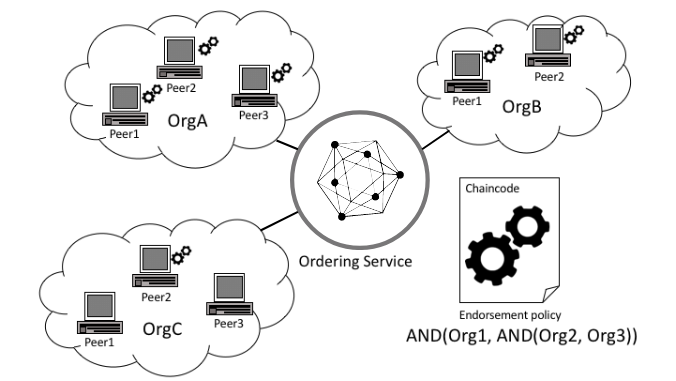
\includegraphics[width=.7\textwidth,height=.35\textwidth]{img/HF.png}
            % \caption{Hyperledger Fabric}
            % \label{fig:arOv}
        \end{figure}}
\end{frame}

\begin{frame}{InterPlanetary File System}{Definition}
    \begin{block}{IPFS}
        InterPlanetary File System, IPFS for short, is a peer-to-peer distributed file system for storing and sharing hypermedia files over a network.
    \end{block}
    \pause
    \begin{figure}
        \centering
        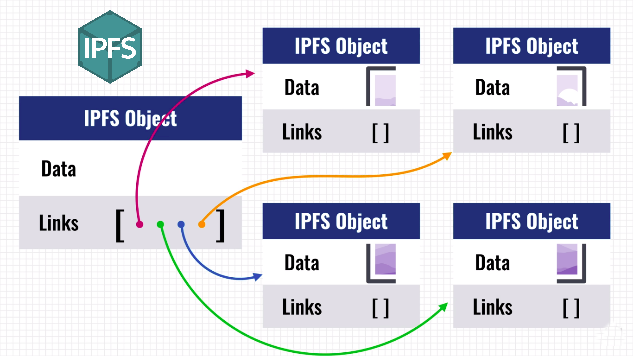
\includegraphics[width=.7\textwidth,height=.35\textwidth]{img/IPFS.png}
        % \caption{InterPlanetary File System}
        % \label{fig:arOv}
    \end{figure}
\end{frame}
